% The Sustainable Development Goals for Tucson 2019 report.
% Author: Dan Stormont
% Organization: Sustainable Tucson

\documentclass[11pt]{book}

% Include packages needed for document
\usepackage{graphicx}

% Build the report.
\begin{document}
\frontmatter

\begin{titlepage}
	\centering
	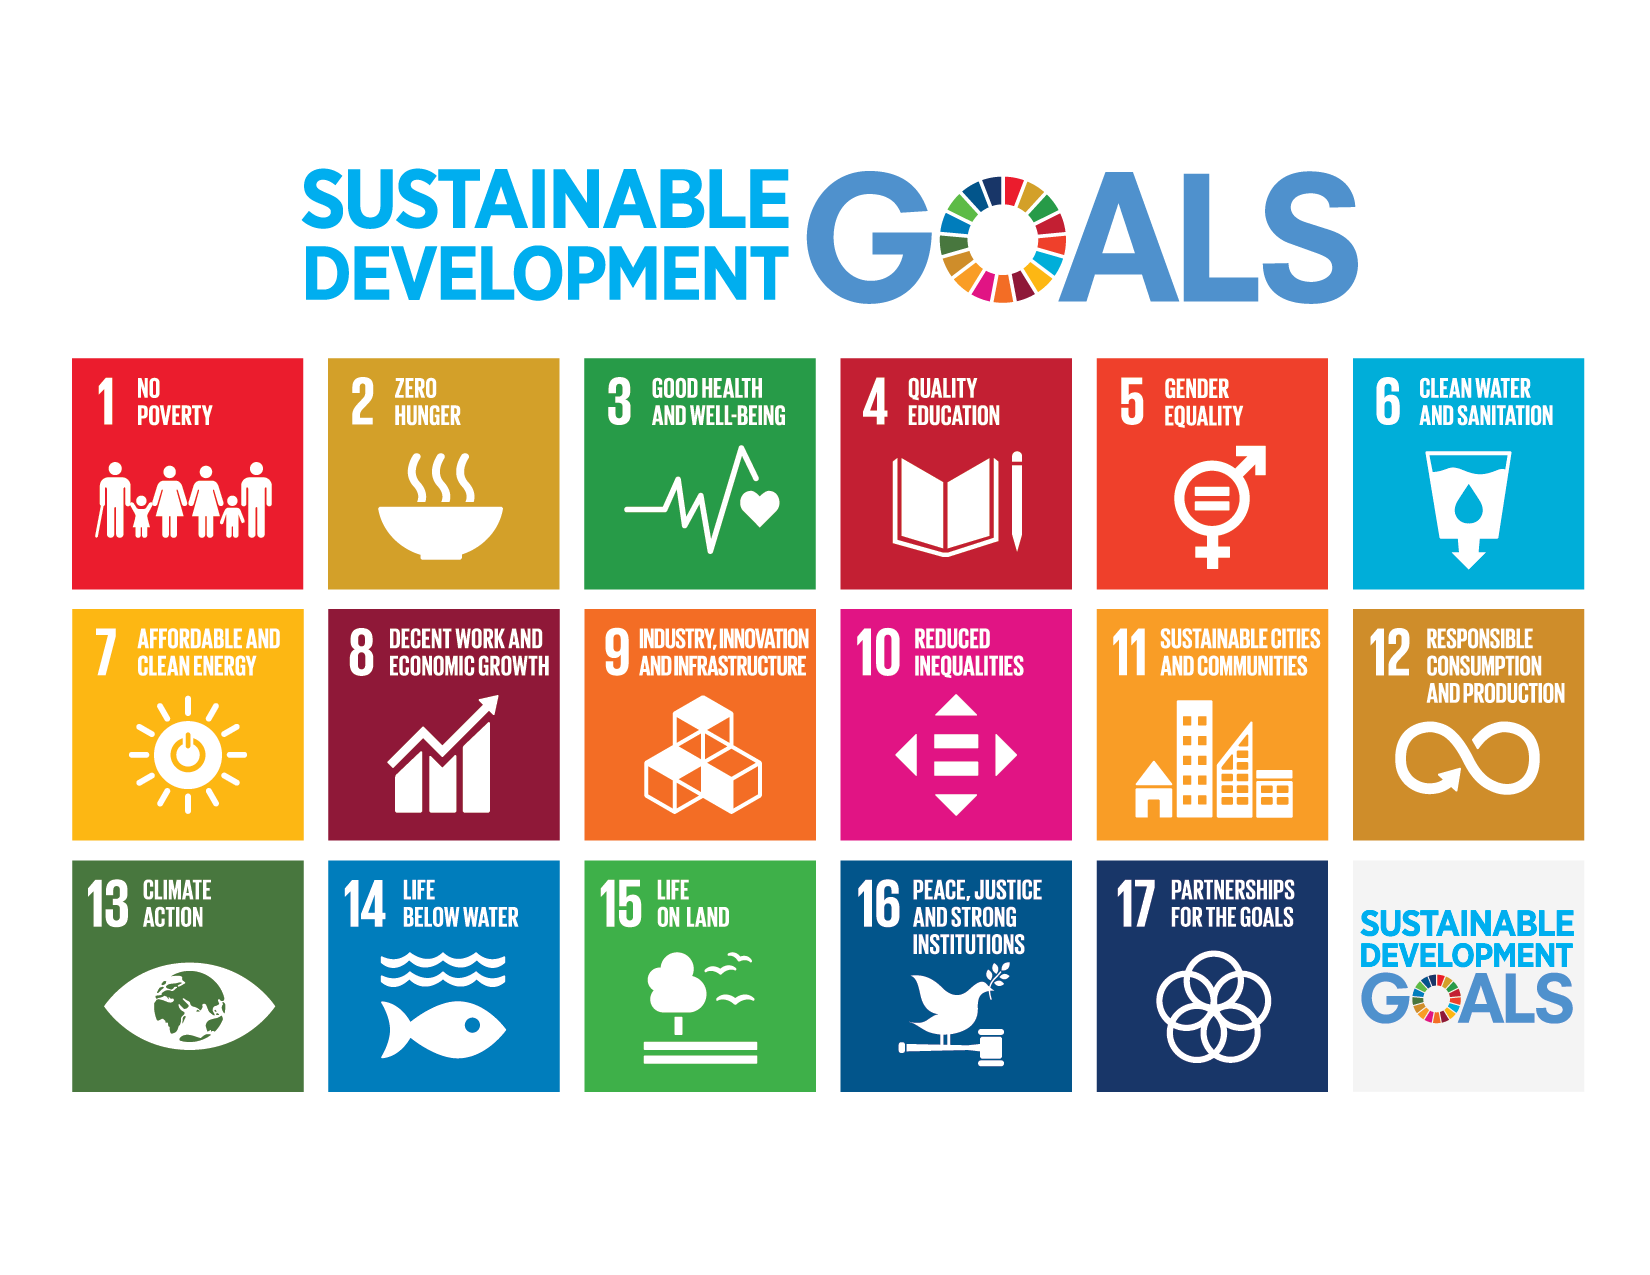
\includegraphics[width=1.0\textwidth]{images/sdg-poster.png}\par
	{\scshape\LARGE Tucson Status Report 2019 \par}
	\vspace{1.5cm}
	
\includegraphics[width=0.3\textwidth]{images/st-logo.jpg}\par
	\vfill
	{\large\today\par}
\end{titlepage}
	
\chapter{The Sustainable Development Goals}

	\section{History}

	\section{Status of the SDGs}

	\section{Why SDGs for Tucson?}

\tableofcontents

\mainmatter

\chapter{Sustainable Development Goal 1: No Poverty}

\Large End poverty in all its forms everywhere.

	\section{National Targets}
	
	\begin{enumerate}
		\item By 2030, eradicate extreme poverty for all people everywhere, currently measured as people living on less than 1.25 a day.
		\item By 2030, reduce at least by half the proportion of men, women, and children of all ages living in poverty in all its dimensions, according to national definitions.
		\item Implement nationally appropriate social protection systems and measures for all, including floors, and by 2030 achieve substantial coverage of the poor and the vulnerable.
		\item By 2030, ensure that all men and women, in particular the poor and the vulnerable, have equal rights to economic resources, as well as access to basic services, ownership and control over land and other forms of property, inheritance, natural resources, appropriate new technology, and financial services, including microfinance.
		\item By 2030, build the resilience of the poor and those in vulnerable situations and reduce their exposure and vulnerability to climate-related extreme events and other economic, social, and environmental shocks and disasters.
	\end{enumerate}

	\section{International Cooperation Targets}
	
	\begin{enumerate}
		\item Ensure significant mobilization of resources from a variety of sources, including through enhanced development cooperation, in order to provide adequate and predictable means for developing countries, in particular least developed countries, to implement programs and policies to end poverty in all its dimensions.
		\item Create sound policy frameworks at the national, regional, and international levels, based on pro-poor and gender-sensitive development strategies, to support accelerated investment in poverty eradication actions.
	\end{enumerate}

	\section{Application of National Targets to Tucson}
	
	\begin{enumerate}
		\item By 2030, eradicate extreme poverty for all people in Tucson, measured as people living at or below 50\% of the Tucson median income.
		\item By 2030,
	\end{enumerate} 

\chapter{Sustainable Development Goal 2: Zero Hunger}

\chapter{Sustainable Development Goal 3: Good Health and Well-Being}

\chapter{Sustainable Development Goal 4: Quality Education}

\chapter{Sustainable Development Goal 5: Gender Equality}

\chapter{Sustainable Development Goal 6: Clean Water and Sanitation}

\chapter{Sustainable Development Goal 7: Affordable and Clean Energy}

\chapter{Sustainable Development Goal 8: Decent Work and Economic Growth}

\chapter{Sustainable Development Goal 9: Industry, Innovation and Infrastructure}

\chapter{Sustainable Development Goal 10: Reduced Inequalities}

\chapter{Sustainable Development Goal 11: Sustainable Cities and Communities}

\chapter{Sustainable Development Goal 12: Responsible Consumption and Production}

\chapter{Sustainable Development Goal 13: Climate Action}

\chapter{Sustainable Development Goal 14: Life Below Water}

\chapter{Sustainable Development Goal 15: Life on Land}

\chapter{Sustainable Development Goal 16: Peace, Justice and Strong Institutions}

\chapter{Sustainable Development Goal 17: Partnerships for the Goals}

\end{document}